\chapter{Introduzione}
\introduction{G. Cutolo}{}

\newpage

\section{Sulle versioni del documento}

\warning{Attento}{
	\textbf{Esistono diverse versioni di questo documento in circolazione}. È fondamentale assicurarsi di \textbf{consultare sempre la versione più recente}, in quanto potrebbe contenere informazioni aggiornate o correzioni rispetto alle versioni precedenti. Per evitare di studiare da fonti non esatte si raccomanda vivamente di verificare la data di pubblicazione e il numero di revisione riportati alla fine di questa pagina.
}

\begin{minipage}{.45\textwidth}
	\begin{center}
		\begin{tblr}{
			colspec = {c|c},
			hlines,
			vlines,
			row{1} = {font=\bfseries, primary!80},
			width = \linewidth
		}
		Revisione & Data \\
		\SetRow{red9} 67dfc7c & 15/03/2024 \\
		\SetRow{red9} 00a8221 & 28/08/202 \\
		\SetRow{red9} 343cc71 & 29/08/2024  \\
		\SetRow{red9}9087dcf & 11/09/2024  \\
		\SetRow{yellow9} 83a3f0f & 01/10/2024 \\
		\SetRow{green9} 3af1354 & 19/02/2025 
	\end{tblr}
	\captionof{table}{Cronologia revisioni del documento}
	\end{center}
\end{minipage}
\hfil
\begin{minipage}{.45\textwidth}
	\begin{center}
		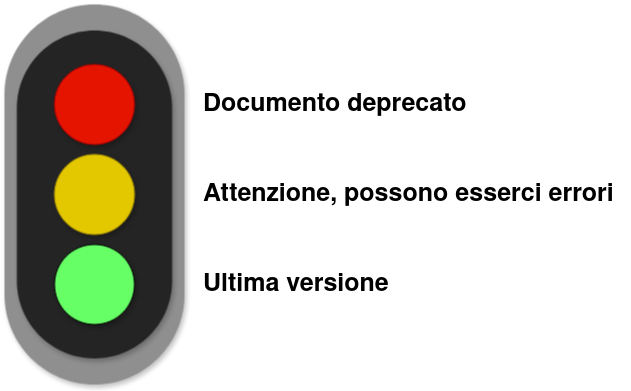
\includegraphics[scale=.35]{sources/Semaforo.drawio}
	\end{center}
\end{minipage}

\section{In caso di errori}
È sempre ben gradito ricevere feedback.

\textbf{Feedback generali:} se hai domande rispetto qualsiasi aspetto del libro non esitare a contattarmi: 
\begin{itemize}
	\item Email: \texttt{giorgio99difusco@gmail.com} 
\end{itemize}

\textbf{Errori:} anche se ti assicuro di aver fatto il massimo per fornirti un documento accurato e preciso, gli errori capitano. Se hai trovato un errore nel libro o vorresti suggerire un miglioramento, sarei grato se me lo potessi segnalare compilato il form che puoi raggiungere seguendo il seguente QR code oppure visitando il seguente \href{https://docs.google.com/spreadsheets/d/1pE-LFclMiIKvmm-tN60bY82P5vNwiK-qvNsq407FNAc/edit?usp=sharing}{link}.

\begin{center}
	
\includegraphics[scale=0.075]{res/Segnalazione_Errori}
\end{center}